\newpage
\section{Предложенный метод}
\label{sec:proposed_method}

В данном разделе представлено описание разработанного алгоритма для визуализации базового представления SCom Tree \cite{garifullin2025compact} с помощью метода извлечения поверхности Marching Cubes \cite{lorensen1987marching} и последующей её растеризации. Алгоритм можно разделить на следующие последовательные этапы:
\begin{enumerate}
    \item Формирование массива активных узлов SCom Tree \cite{garifullin2025compact} (см. разд. \ref{ssec:active_leafs})
    \item Извлечение поверхности из вокселей алгоритмом \cite{lorensen1987marching} (см. разд. \ref{ssec:marching_cubes})
    \item Растеризация в буферы геометрии (см. разд. \ref{ssec:raster})
    \item Постобработка и расчёт освещения (см. разд. \ref{ssec:postprocessing})
    \item Заполнение Hi-Z буфера (см. разд. \ref{ssec:hz_buffer}) для использования в следующем кадре
\end{enumerate}

\subsection{Формирование массива активных узлов} \label{ssec:active_leafs}

Первым этапом является идентификация тех фрагментов пространства, которые делают вклад в получаемое изображение. Качественная реализация этого этапа минимизирует работу последующих, отсекая при формировании списка листовых узлов целые поддеревья иерархии без необходимости обходить всю структуру целиком. Являясь начальным, этот этап \textbf{принимает на вход непосредственно структуру SCom Tree \cite{garifullin2025compact}} --- таким образом, предложенный метод реализует прямой рендеринг этого компактного представления трёхмерной модели без предварительной распаковки и извлечения поверхности.

\begin{figure}[ht!]
    \centering
    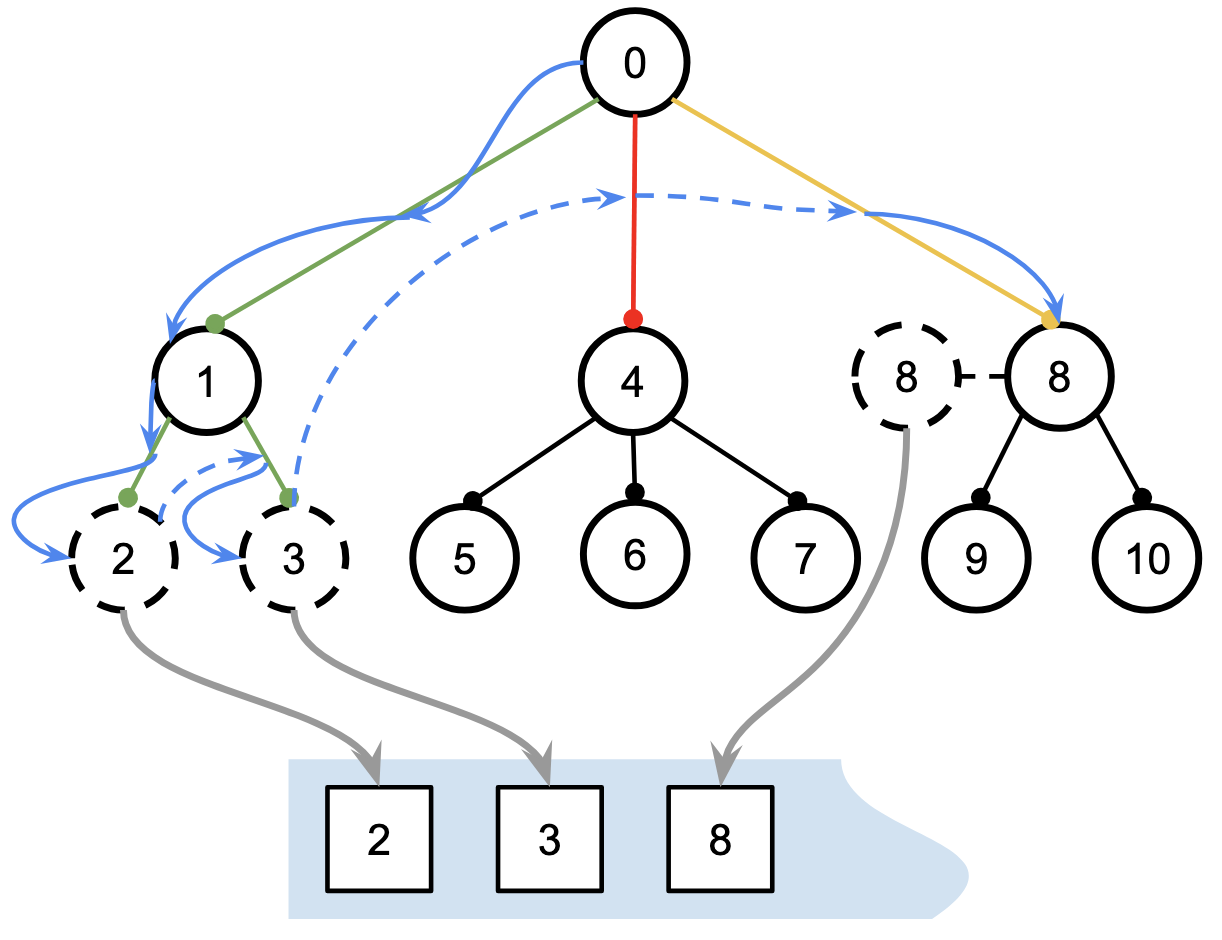
\includegraphics[width=0.7\textwidth]{figures/dfs.png} 
    \caption{\textbf{Схема вариации алгоритма обхода в глубину для поиска активных узлов.} Синими стрелками обозначен маршрут обхода иерархии, пунктирными -- момент когда нам потребовалось обратиться к стеку с ребрами ''на очереди'' (например при спуске по ребру 0-1 в стек кладется ребро 0-4). В ребрах происходит проверка: спуск необходим (зелёный), спуск не требуется (красный), спуск требуется, с условием, что узел ''станет листовым'' (жёлтый). Серым обозначены атомарные операции добавления активного узла в массив. На схеме изображены только непустые узлы октодерева, описывающие геометрию модели.}
    \label{fig:dfs}
\end{figure}

Алгоритм \ref{fig:dfs} обходит иерархическую древовидную структуру SCom Tree \cite{garifullin2025compact} в глубину, то есть всегда выбирая спуститься глубже по структуре, вместо того чтобы сразу разбираться со всеми узлами текущего уровня иерархии. В качестве вспомогательной структуры данных для алгоритма используется стек.

\newpage
Для принятия решения о спуске к дочерним узлам или отсечении текущей ветви дерева выполняются три последовательные проверки.

\paragraph{Отсечение фрустумом (Frustum Culling)} 
Узел отбрасывается (см. узел 4 на рис. \ref{fig:dfs}), если его воксель полностью находится за пределами пирамиды видимости \cite[с. 835]{RTR4}. Для проверки пересечения используется алгоритм SAT (Separating Axis Theorem), согласно которому два выпуклых многогранника не пересекаются, если существует хотя бы одна ось, на которую проекции этих объектов не накладываются друг на друга. Если такая ось найдена, поддерево исключается из дальнейшего обхода.

\paragraph{Окклюзионное отсечение (Occlusion Culling)} 
Узел отбрасывается, если он полностью перекрыт более близкой к камере геометрией. Для этого ограничивающий объем (AABB) узла проецируется на экранную плоскость. С помощью иерархического буфера глубины (Hi-Z), сформированного на предыдущем кадре (см. разд. \ref{ssec:hz_buffer}), выполняется сравнение минимальной глубины узла с максимальной глубиной в соответствующей области Hi-Z буфера.

\paragraph{Уровень детализации (Level of Detail)} 
Спуск по дереву прекращается, если текущий уровень узла $L_{curr}$ обеспечивает достаточную визуальную точность. Сначала вычисляется размер проекции эталонного объема в экранном пространстве ($P_{px}$):

\begin{equation}
P_{px} = \frac{S_{world} \cdot H_{screen}}{2 \cdot d_{min} \cdot \tan\left(\frac{f_{FOV}}{2}\right)}
\end{equation}

где $S_{world}$ — константа мирового масштаба ($2.0$), $H_{screen}$ — высота экрана в пикселях, $d_{min}$ — расстояние от камеры до AABB узла, а $f_{FOV}$ — вертикальный угол обзора. На основе полученного значения вычисляется целевая глубина детализации $L_{target}$:

\begin{equation}
L_{target} = 
\begin{cases} 
0, & P_{px} \le T_{px} \\
\log_2 \left( \frac{P_{px}}{T_{px}} \right) \cdot k, & P_{px} > T_{px}
\end{cases}
\end{equation}

здесь $T_{px}$ — порог детализации в пикселях, а $k$ — коэффициент агрессивности LOD. Использование константного $S_{world}$ делает расчет независимым от текущего размера узла, обеспечивая стабильность иерархии при перемещении камеры. Если $L_{curr} \ge L_{target}$, узел помечается как листовой активный узел (узел 8 на рис. \ref{fig:dfs}), и дальнейший обход его потомков не производится.

\textbf{Результатом данного этапа является линейный массив активных узлов}, каждый из которых представляет собой кубическую область пространства определенного уровня детализации. Использование линейного массива на выходе позволяет эффективно распределять нагрузку на последующих стадиях.

\subsection{Триангуляция поверхности} \label{ssec:marching_cubes}

После того как список активных узлов сформирован, выполняется локальное извлечение поверхности внутри каждого кубического пространства, соответствующего им. В статье под авторством Garifullin \cite{garifullin2025compact} эти кубические пространства называют "бриками" или "кирпичиками". Каждый из этих "бриков" хранит в себе небольшую декартову решетку, в узлах которой определены значения функции SDF. В предложенном методе число значений на ось решетки равно 3, таким образом число вокселей для алгоритма Marching Cubes \cite{lorensen1987marching} равно 8.

\begin{figure}[ht!]
    \centering
    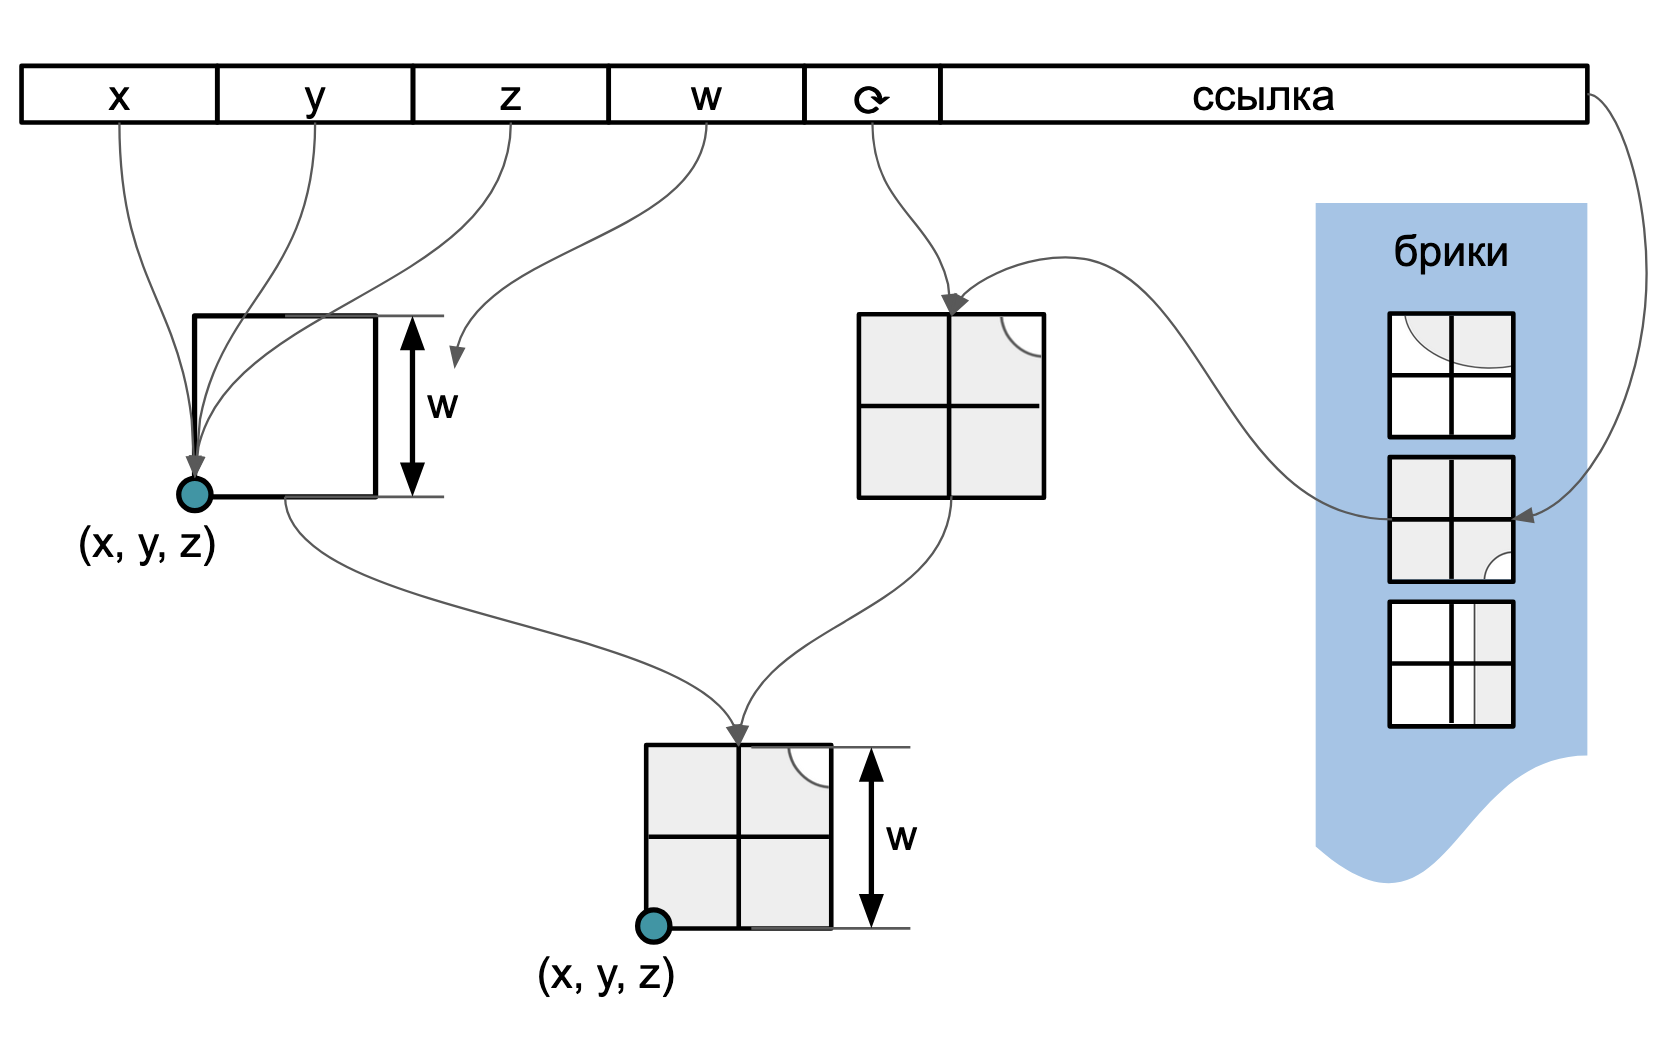
\includegraphics[width=\textwidth]{figures/unpack_brick.png} 
    \caption{Иллюстрация на плоскости процесса получения вокселей для Marching Cubes из активного узла.}
    \label{fig:unpack_brick}
\end{figure}

Процесс триангуляции для каждого вокселя включает:
\begin{itemize}
    \item \textbf{Выборку значений SDF:} В восьми вершинах кубического узла вычисляются (или извлекаются из структуры данных) значения знаковой функции расстояния.
    \item \textbf{Интерполяцию позиций вершин:} Если значения SDF в соседних вершинах имеют разные знаки, это означает, что поверхность пересекает ребро между ними. Точное положение вершины треугольника $P$ на ребре $(P_1, P_2)$ вычисляется с помощью линейной интерполяции:
    \begin{equation}
        P = P_1 + (P_2 - P_1) \cdot \frac{0 - SDF(P_1)}{SDF(P_2) - SDF(P_1)}
    \end{equation}
    \item \textbf{Генерацию нормалей:} В каждой извлеченной вершине вычисляется вектор нормали к поверхности как нормированный градиент SDF. Применение метода центральных разностей позволяет получить гладкие нормали даже для дискретных представлений.
\end{itemize}

Итогом этапа является набор треугольников, локально аппроксимирующих неявную поверхность с заданной точностью.

\subsection{Растеризация} \label{ssec:raster}

Сгенерированные на предыдущем этапе треугольники подаются на вход стандартного этапа растеризации. Здесь применяется концепция \textit{отложенного рендеринга} (Deferred Rendering) и использование G-буфера (Geometry Buffer), потому что это необходимо для постобработки (см. разд. \ref{sec:postprocessing}).

Растеризатор преобразует трехмерные треугольники в двумерные фрагменты (пиксели), заполняя G-буфер следующими данными:
\begin{itemize}
    \item \textbf{Мировые координаты, вектор нормали и цвет:} Используется в \ref{alg:blinn_phong}.
    \item \textbf{Глубина:} Используется в \ref{alg:fix_depth}.
\end{itemize}

\subsection{Постобработка и расчёт освещения} \label{ssec:postprocessing}

На этом этапе выполняется расчет итогового цвета каждого пикселя на основе данных из G-буфера. Этот этап включает 3 ключевых шага:
\begin{enumerate}
    \item \textbf{Коррекция визуальной связности:} Алг
    \item \textbf{Расчет освещения:} Применение моделей освещения (например, модели Фонга или PBR) с использованием нормалей и позиций из G-буфера.
    \item \textbf{Заполнение базового Mip изображения Hi-Z буфера:} Алг
\end{enumerate}

\subsubsection{Коррекция визуальной связности}

\begin{figure}[ht!]
    \centering
    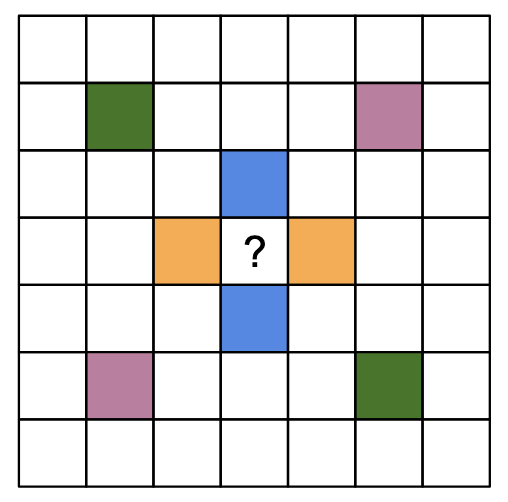
\includegraphics[width=0.3\textwidth]{figures/fix_depth.png} 
    \caption{Паттерн сэмплирования значений буфера глубины для восстановления визуальной связности.}
    \label{fig:fix_depth}
\end{figure}

Для обнаружения локальных разрывов глубины используется метод многонаправленного анализа окрестностей (рис. \ref{fig:fix_depth}), в рамках которого центральный пиксель сравнивается с четырьмя парами симметричных соседей: по горизонтали и вертикали (шаг 1 пкс), а также по диагоналям (шаг 2 пкс). Пиксель идентифицируется как артефакт («дыра»), если по любой из указанных осей он существенно глубже своих соседей при условии их взаимной топологической близости.

\begin{algorithm}[H]
    \SetAlFnt{\small\rmfamily}
    \SetAlCapFnt{\small\rmfamily}
    \SetAlCapNameFnt{\small\rmfamily}

    \KwIn{
        $\mathbf{pos}$ — позиция фрагмента; 
        $\mathbf{N}$ — нормаль; 
        $\mathbf{C}_{alb}$ — альбедо; \\
        $\mathbf{light\_pos}$ — позиция источника света; 
        $\mathbf{camera\_pos}$ — позиция камеры; \\
        $\mathbf{C}_{light}$ — цвет источника света; 
        $k_{amb}, k_{spec}$ — коэффициенты освещения; 
        $p$ — степень блеска
    }
    \KwOut{$\mathbf{C}_{final}$ — итоговый цвет пикселя}

    \BlankLine
    $\mathbf{L} \leftarrow \text{normalize}(\mathbf{light\_pos} - \mathbf{pos})$\;
    $\mathbf{V} \leftarrow \text{normalize}(\mathbf{camera\_pos} - \mathbf{pos})$\;
    $\mathbf{H} \leftarrow \text{normalize}(\mathbf{L} + \mathbf{V})$\;

    \BlankLine
    $\mathbf{I}_{amb} \leftarrow \mathbf{C}_{alb} \cdot k_{amb}$\;

    \BlankLine
    $diff \leftarrow \max(\mathbf{N} \cdot \mathbf{L}, 0.0)$\;
    $\mathbf{I}_{diff} \leftarrow \mathbf{C}_{alb} \cdot diff \cdot \mathbf{C}_{light}$\;

    \BlankLine
    $spec \leftarrow \max(\mathbf{N} \cdot \mathbf{H}, 0.0)^{p}$\;
    $\mathbf{I}_{spec} \leftarrow k_{spec} \cdot spec \cdot \mathbf{C}_{light}$\;

    \BlankLine
    $\mathbf{C}_{final} \leftarrow \mathbf{I}_{amb} + \mathbf{I}_{diff} + \mathbf{I}_{spec}$\;
    \Return $\mathbf{C}_{final}$\;

    \caption{Расчёт освещения (Blinn-Phong)}
    \label{alg:blinn_phong}
\end{algorithm}

\subsection{Заполнение Hi-Z буфера} \label{ssec:hz_buffer}

Для эффективной проверки видимости узлов октодерева используется иерархическое представление буфера глубины (Hi-Z), позволяющее выполнять консервативный тест на окклюзию для объектов произвольного размера. Hi-Z буфер представляет собой пирамиду текстур (mip-levels), где каждый пиксель уровня $i$ содержит максимальное значение глубины соответствующих ему пикселей уровня $i-1$ \ref{fig:hz_buffer}.

\begin{figure}[ht!]
    \centering
    
\includegraphics[width=0.5\textwidth]{figures/hz_buffer.png} 
    \caption{Пример первых трех mip уровней Hi-Z буфера.}
    \label{fig:hz_buffer}
\end{figure}

Нулевой уровнь (mip 0) Hi-Z буфера заполняется еще на предыдущем этапе (см. разд. \ref{ssec:postprocessing}). Построение последующих уровней выполняется итеративно. Для каждого уровня $i > 0$ запускается алгоритм \ref{alg:hz_buffer}, который использует окрестность пикселей $3 \times 3$ для обеспечения консервативности. Это гарантирует, что если хотя бы один фрагмент геометрии на детальном уровне был ближе к камере, это значение «всплывет» на верхние уровни иерархии, предотвращая ложные срабатывания теста видимости.

\begin{algorithm}[H]
    \SetAlFnt{\small\rmfamily}
    \SetAlCapFnt{\small\rmfamily}
    \SetAlCapNameFnt{\small\rmfamily}

    \KwIn{
        $id$ --- индекс потока; \\
        $src\_tex, dst\_tex$ --- исходная и целевая текстуры; \\
        $src\_res, dst\_res$ --- разрешения уровней.
    }
    \KwOut{$dst\_tex[dst\_coord]$ — обновленное значение Hi-Z буфера}

    \BlankLine
    $dst\_coord \leftarrow id.xy$\;

    \If{$dst\_coord.x \ge dst\_res.x$ \textbf{or} $dst\_coord.y \ge dst\_res.y$}{
        \Return\;
    }

    \BlankLine
    $scale \leftarrow (src\_res / dst\_res)$\;
    $src\_center \leftarrow \text{ceil}(dst\_coord \cdot scale)$\;
    $max\_depth \leftarrow 0.0$\;

    \BlankLine
    \For{$y \leftarrow -1$ \KwTo $1$}{
        \For{$x \leftarrow -1$ \KwTo $1$}{
            $coords.x \leftarrow \text{clamp}(src\_center.x + x, 0, src\_res.x - 1)$\;
            $coords.y \leftarrow \text{clamp}(src\_center.y + y, 0, src\_res.y - 1)$\;

            \BlankLine
            $depth \leftarrow src\_tex[coords]$\;
            $max\_depth \leftarrow \max(max\_depth, depth)$\;
        }
    }

    \BlankLine
    $dst\_tex[dst\_coord] \leftarrow max\_depth$\;

    \caption{Генерация Mip-уровня Hi-Z буфера (консервативный фильтр $3 \times 3$)}
    \label{alg:hz_buffer}
\end{algorithm}

\subsection{Програмная реализация} \label{ssec:optimization}
Весь алогритм реализован для работы на графическом процессоре с использованием технологии программирования Vulkan API. Первые два этапа, поиск активных узлов и извлечение поверхности реализованы с помощью вычислительных шейдеров. Второй этап в ходе решения третьей задачи этой работы был также реализован в виде Mesh Shader \cite{nvidia_mesh_shaders}.

Внедрение Mesh Shaders \cite{nvidia_mesh_shaders} убрало потребность выделять в видеопамяти буферы для хранения сгенерированных примитивов. В текущей реализации примитивы, извлеченные из неявной функции алгоритмом Marching Cubes \cite{lorensen1987marching} отправляются в растеризатор напрямую. За счет этого достигается максимальная эффективность графического конвейера: отсутствие промежуточных буферов снижает задержки (latency), а генерация геометрии внутри меш-шейдеров позволяет видеокарте обрабатывать данные локально в быстрой кэш-памяти.

Также, в дополнение к классическому обходу дерева в глубину (Depth First Search) на этапе формирования массива активных листьев (см. разд.~\ref{ssec:active_leafs}) предлагается алгоритм, использующий структурные особенности разреженного октодерева (Sparse Octree), лежащего в основе SCom Tree \cite{garifullin2025compact}. Свойства данной структуры гарантируют, что каждый внутренний узел содержит не более восьми дочерних элементов. 

Использование трехмерной индексации потоков (threads) и рабочих групп (workgroups) в графических процессорах позволяет оптимизировать процесс навигации по дереву. При назначении восьми вычислительных единиц на каждую координатную ось становится доступным спуск на шесть уровней иерархии с минимальными вычислительными затратами: индексы первых трех уровней определяются положением рабочей группы (по осям $x, y, z$ соответственно), а последующие три уровня -- индексами потоков внутри группы.

В случаях, когда дальнейший спуск невозможен -- вследствие отсечения (Frustum, Occlusion Culling), достижения требуемого уровня детализации (LoD) или отсутствия геометрии в узле, -- необходимо исключить избыточность вычислений. Для предотвращения дублирования данных в итоговом массиве активных листьев внедряется механизм раннего завершения потоков: обработку таких узлов продолжают только те потоки, которые соответствуют нулевым индексам в иерархии ветвления. Данный подход гарантирует уникальность каждой записи в целевом буфере и позволяет лучше распределить нагрузку на графический процессор.

Если достигнутый в результате спуска узел не является листовым -- остаток иерархии подвергается изложенному в разд.~\ref{ssec:active_leafs} алгоритму обхода в глубину.

